\chapter{Vì sao siêu đối xứng có thể quan trọng}

\lectureoverview{Các dao động chân không liên kết các chủ đề của chương này.
Các điều kiện biên tạo ra lực Casimir, các hiệu ứng vòng đe dọa khối lượng Higgs,
các hạt ảo mới làm thay đổi sự chạy của các hằng số ghép chuẩn, và năng lượng chân không
chi phối sự giãn nở vũ trụ. Những vấn đề này thúc đẩy việc xét siêu đối xứng năng lượng thấp như
một cách ổn định hóa thang Higgs, cung cấp một ứng viên vật chất tối, và cải thiện
sự hợp nhất các hằng số ghép chuẩn. Sau đó ta xây dựng các siêu trường bằng các tọa độ Grassmann
và dùng tích phân Berezin để rút ra một tác dụng siêu đối xứng.}

\section{Dao động chân không giữa các bản phản xạ}

Ta quay lại siêu đối xứng bằng cách trước hết giải quyết một câu hỏi về hiệu ứng Casimir. Đặt hai bản phản xạ song song cách nhau một khoảng \(d\). Ngay cả khi không có hạt thực nào hiện diện, một trường lượng tử vẫn có các dao động chân không. Ta có thể hình dung chúng như các quá trình ảo, hoặc tương đương, như chuyển động điểm không của các mode dao động của trường. Các bản áp đặt điều kiện biên, nên những dao động được phép giữa chúng khác với trong không gian không bị ràng buộc.

Đại lượng quan trọng không phải là mốc không tuyệt đối của năng lượng mà là độ biến thiên sinh ra khi khoảng cách thay đổi. Ký hiệu năng lượng chân không trên một đơn vị diện tích là \(\mathcal E(d)=E(d)/A\). Một khi \(\mathcal E\) phụ thuộc vào \(d\), nó là thế năng, và lực trên một đơn vị diện tích là
\begin{equation}
\frac{F}{A}=-\frac{d\mathcal E}{dd}.
\end{equation}
Vì thế sự sắp xếp lại của các quá trình ảo trở thành một lực quan sát được. Trong ví dụ điện từ quen thuộc với các bản dẫn lý tưởng, năng lượng và áp suất là
\begin{align}
\mathcal E(d)&=-\frac{\pi^2}{720\,d^3},\\
\frac{F}{A}&=-\frac{\pi^2}{240\,d^4},
\end{align}
trong đơn vị \(\hbar=c=1\).\editorialnote{Các hệ số này và sự phân biệt giữa năng lượng trên một đơn vị diện tích \(d^{-3}\) và áp suất \(d^{-4}\) giải quyết câu hỏi về thứ nguyên được nêu trên bảng. Đây là kết quả chuẩn cho các bản lý tưởng, không phải là một phép dẫn xuất được trình bày ở đây.} Dấu trừ biểu thị lực hút.

\begin{classroomqa}
\audiencequestion{Lũy thừa bậc bốn mô tả lực hay năng lượng? \lecturetimestamp{00:04:39}}
\lecturerresponse{Đối với các bản song song trong không-thời gian bốn chiều, năng lượng trên một đơn vị diện tích giảm như \(d^{-3}\), còn khi lấy đạo hàm theo \(d\) thì lực trên một đơn vị diện tích giảm như \(d^{-4}\). Phân tích thứ nguyên đã xác định sẵn các lũy thừa này một khi khôi phục \(\hbar\) và \(c\).}
\end{classroomqa}

Đôi khi người ta tóm tắt phép tính bằng cách nói rằng các bản làm gián đoạn các vòng photon ảo. Hình ảnh đó hữu ích miễn là không hiểu quá theo nghĩa đen. Phép tính chính xác là sự thay đổi trong phổ các mode trường được phép hoặc, tương đương, là sự thay đổi trong tác dụng hiệu dụng lượng tử. Cả hai ngôn ngữ đều dẫn đến cùng một năng lượng phụ thuộc vào khoảng cách.

\begin{classroomqa}
\audiencequestion{Lực Casimir có thể là lực đẩy thay vì lực hút không? \lecturetimestamp{00:07:48}}
\lecturerresponse{Có thể. Dấu của nó không mang tính phổ quát; nó phụ thuộc vào các trường, hình học, vật liệu và điều kiện biên. Các vòng fermion thường mang dấu vòng ngược với các vòng boson, điều này gợi ý đề xuất được nêu trên bảng, nhưng riêng thống kê fermion tự nó không phải là một định lý tổng quát rằng mọi lực Casimir đều phải là lực đẩy.\editorialnote{Sự lưu ý này thay thế một câu trả lời trên lớp được cố ý nói dè dặt bằng phát biểu tổng quát cần thiết để tránh một quy tắc phổ quát sai.}}
\end{classroomqa}

\subsection{Điều gì sẽ được xem là bằng chứng cho năng lượng chân không?}

Lực Casimir đã được đo, và các đại lượng quan sát nguyên tử cũng nhạy với các vòng chân không. Tuy nhiên, tự thân không điều nào trong hai điều ấy chứng tỏ rằng một năng lượng chân không tuyệt đối có hấp dẫn. Một thí nghiệm Casimir đo một độ chênh năng lượng do điều kiện biên gây ra; cùng lực ấy có thể được mô tả mà không cần gán ý nghĩa thao tác cho một tổng tuyệt đối các năng lượng điểm không không bị chặn.

Phép kiểm tra quyết định đến từ hấp dẫn. Năng lượng là điện tích hấp dẫn. Nếu không gian trống mang một mật độ năng lượng đồng đều, nó phải đi vào các phương trình Einstein và ảnh hưởng đến sự giãn nở vũ trụ. Vì vậy sự giãn nở gia tốc của vũ trụ là bằng chứng hấp dẫn trực tiếp cho một thành phần kiểu chân không.

\begin{classroomqa}
\audiencequestion{Vì sao các trình bày phổ thông gọi năng lượng chân không là bí ẩn, như thể các nhà vật lý không biết nó là gì? \lecturetimestamp{00:08:19}}
\lecturerresponse{Lý thuyết trường lượng tử gán cho mọi trường một đóng góp điểm không, nên khả năng tồn tại năng lượng chân không không phải là điều bí ẩn. Điều bí ẩn nằm ở mặt định lượng: vì sao giá trị hấp dẫn của nó lại nhỏ đến phi thường so với các ước lượng dựa trên những trường lượng tử đã biết và một ngưỡng cắt năng lượng cao? Sự thật gây ngạc nhiên là nó gần như vắng mặt, chứ không phải sự hiện diện đơn thuần của nó.}
\end{classroomqa}

Trong nhiều năm, cận trên quan sát nhỏ đến mức về mặt tâm lý người ta dễ bị cám dỗ đặt hằng số vũ trụ học đúng bằng không và tìm một nguyên lý cưỡng bức sự triệt tiêu ấy. Thay vào đó, các quan sát vũ trụ học được cải thiện đã tìm thấy một giá trị nhỏ nhưng khác không. Phát hiện đó không khiến năng lượng chân không trở nên xa lạ về mặt khái niệm; nó khiến mức độ bị triệt tiêu chưa được giải thích trở nên không thể phớt lờ. Phép so sánh thích hợp phụ thuộc vào thang tử ngoại được giả định, nhưng mọi ước lượng năng lượng cao tự nhiên đều đòi hỏi một sự triệt tiêu khổng lồ.

\section{Một siêu điện tích tác động lên một trạng thái nhiều hạt như thế nào}

Trước khi liệt kê các lý do để tin vào siêu đối xứng, ta nên loại bỏ một nghịch lý có thể có. Boson có thể cùng chiếm một mode với số lượng lớn tùy ý, trong khi một mode fermion có số chiếm bằng không hoặc một. Nếu một đối xứng hoán đổi boson và fermion, liệu nó có biến một nghìn boson trong một mode thành một nghìn fermion bị cấm không?

Không. Một bộ sinh fermion thay đổi mỗi lần một lượng tử. Trong mô hình dao động tử, cho \(a\) hủy một boson và \(c^\dagger\) tạo ra đối tác fermion của nó. Một siêu điện tích có thể được biểu diễn bởi
\begin{equation}
Q=c^\dagger a.
\end{equation}
Trên một trạng thái có \(n\) boson và không có fermion,
\begin{equation}
Q\ket{n,0}
=\sqrt n\,\ket{n-1,1}.
\end{equation}
Một boson đã bị lấy đi và một fermion được đưa vào. Tác dụng lần nữa với cùng điện tích cho kết quả bằng không:
\begin{equation}
Q^2=(c^\dagger)^2a^2=0.
\end{equation}
Đây là tính lũy linh kế thừa từ các toán tử tạo fermion.

\begin{classroomqa}
\audiencequestion{Nếu nhiều boson cùng chiếm một trạng thái, vì sao một phép biến đổi siêu đối xứng không tạo ra nhiều fermion trong chính trạng thái ấy và vi phạm nguyên lý loại trừ? \lecturetimestamp{00:12:05}}
\lecturerresponse{Bộ sinh không thay thế toàn bộ số hạt đang chiếm. Nó làm thay đổi trạng thái đi một đơn vị số fermion. Cùng một điện tích fermion không thể được chập lại như một bộ sinh quay thông thường vì bình phương của nó bằng không. Một điện tích bổ sung có thể hoàn tác sự hoán đổi, và phản giao hoán tử hỗn hợp khép trên phép tịnh tiến theo thời gian.}
\end{classroomqa}

Câu cuối cùng là thiết yếu. Ký hiệu tắt \(Q^2=0\) áp dụng cho một thành phần chiral riêng lẻ hoặc cho điện tích đơn giản vừa viết; nó không có nghĩa là mọi tích của các siêu điện tích đều triệt tiêu. Trong siêu đối xứng bốn chiều,
\begin{equation}
\{Q_\alpha,\bar Q_{\dot\beta}\}
=2\sigma^\mu_{\alpha\dot\beta}P_\mu,
\end{equation}
còn
\begin{equation}
\{Q_\alpha,Q_\beta\}=0,
\qquad
\{\bar Q_{\dot\alpha},\bar Q_{\dot\beta}\}=0
\end{equation}
đối với đại số tối thiểu không có điện tích trung tâm.\editorialnote{Dạng theo thành phần này phát biểu chính xác lối nói tắt trên lớp rằng việc tác dụng lặp lại của cùng một \(Q\) sẽ triệt tiêu, trong khi một siêu điện tích và liên hợp của nó sinh ra phép tịnh tiến.}

\section{Ba lý do để tìm kiếm siêu đối xứng năng lượng thấp}

\begin{classroomqa}
\audiencequestion{Ngoài việc triệt tiêu năng lượng chân không, còn có động lực nào cho siêu đối xứng không? \lecturetimestamp{00:15:06}}
\lecturerresponse{Có ba động lực gắn bó chặt chẽ với nhau: kiểm soát tự năng lượng của Higgs, một hạt vật chất tối ổn định khả dĩ, và sự gặp nhau sắc nét hơn nhiều của các hằng số ghép chuẩn ở năng lượng cao. Không điều nào chứng minh rằng siêu đối xứng được thực hiện trong tự nhiên, nhưng gộp lại chúng khiến nó trở thành một lý thuyết nghiêm túc cần được kiểm nghiệm.}
\end{classroomqa}

Cụm từ \emph{siêu đối xứng năng lượng thấp} mang tính tương đối. Nó không có nghĩa là các siêu đối tác nhẹ theo thang đo đời thường; nó có nghĩa là khối lượng của chúng không lớn vượt xa thang điện yếu và thang của máy gia tốc. Cả ba lập luận đều yếu đi nếu các siêu đối tác bị đẩy lên cao tùy ý.

\subsection{Bảo vệ thang Higgs}

Khối lượng của một trường vô hướng nhạy một cách khác thường với vật lý năng lượng cao. Về sơ đồ, một vòng boson tạo ra một hiệu chỉnh có dạng
\begin{equation}
\delta m_H^2\big|_{\mathrm B}
\sim +\frac{\lambda}{16\pi^2}\Lambda^2,
\end{equation}
trong đó \(\Lambda\) ký hiệu thang mà đến đó lý thuyết hiệu dụng đang được dùng. Một vòng fermion mang dấu ngược lại,
\begin{equation}
\delta m_H^2\big|_{\mathrm F}
\sim -\frac{|y|^2}{8\pi^2}\Lambda^2.
\end{equation}
Các hệ số phụ thuộc vào tương tác và bội số của các trường, nhưng siêu đối xứng liên hệ chúng với nhau sao cho độ nhạy tử ngoại bậc dẫn triệt tiêu giữa các đối tác.\editorialnote{Các công thức vòng sơ đồ này bộc lộ toán học đứng sau lập luận định tính về tự năng lượng. Chúng không nhằm trở thành một phép tính đầy đủ khối lượng Higgs trong Mô hình Chuẩn.}

Điều này quan trọng vì giá trị kỳ vọng của Higgs đặt ra thang điện yếu. Khối lượng của boson chuẩn và fermion tuân theo các hệ thức như
\begin{equation}
m_W=\frac{gv}{2},
\qquad
m_f=\frac{y_fv}{\sqrt2}.
\end{equation}
Nếu khu vực Higgs một cách tự nhiên bị đẩy lên một thang khổng lồ, phổ hạt năng lượng thấp quen thuộc sẽ mất đi trừ khi các tham số trần được điều chỉnh bù với các hiệu chỉnh bức xạ bằng độ chính xác cực cao.

Siêu đối xứng chính xác sẽ làm cho sự triệt tiêu là chính xác, nhưng siêu đối xứng chính xác đã bị loại trừ bởi khối lượng không bằng nhau của các boson và fermion quan sát được. Với siêu đối xứng bị phá vỡ mềm, độ nhạy bậc hai được thay bằng sự phụ thuộc vào độ tách khối lượng giữa các siêu đối tác, một cách sơ đồ
\begin{equation}
\delta m_H^2
\sim
\frac{g^2}{16\pi^2}
\left(m_{\mathrm{soft}}^2-m_{\mathrm{ordinary}}^2\right)
\ln\frac{\Lambda^2}{m_{\mathrm{soft}}^2}.
\end{equation}
Sự triệt tiêu chỉ còn hữu ích chừng nào độ tách ấy chưa quá lớn.

\subsection{Một điểm cuối ổn định cho các chuỗi phân rã vật chất tối}

Hãy tách phổ thành các hạt thông thường và các siêu đối tác của chúng. Một fermion có một đối tác boson; một boson có một đối tác fermion. Nếu các tương tác bảo toàn một đối xứng chẵn lẻ phân biệt hai lớp này, thì một phân rã của siêu đối tác phải để lại một siêu đối tác khác:
\begin{equation}
\widetilde X
\longrightarrow X+\widetilde Y
\longrightarrow X+Y+\widetilde Z
\longrightarrow\cdots.
\end{equation}
Chuỗi phân rã không thể loại bỏ siêu đối tác cuối cùng của nó. Vì vậy nó kết thúc ở hạt siêu đối xứng nhẹ nhất, LSP.

Đối xứng thường dùng là đối tính \(R\),
\begin{equation}
R_p=(-1)^{3(B-L)+2s}.
\end{equation}
Các hạt của Mô hình Chuẩn có \(R_p=+1\), còn các siêu đối tác của chúng có \(R_p=-1\). Nếu \(R_p\) là chính xác, mọi tương tác đều chứa một số chẵn siêu đối tác và LSP là ổn định.\editorialnote{Chỉ riêng siêu đối xứng không bảo đảm một LSP ổn định. Tính ổn định đòi hỏi đối tính \(R\) được bảo toàn hoặc một đối xứng khác có cùng hệ quả; nếu không, LSP có thể phân rã.}

Vật chất tối phải tồn tại ít nhất trên các thang thời gian vũ trụ học. Nó cũng phải tương tác đủ yếu để nhiều lần đi xuyên qua đĩa thiên hà nhìn thấy được mà không mất năng lượng đáng kể. Một quần thể mang điện hoặc tương tác mạnh sẽ tán xạ, tiêu tán năng lượng và có xu hướng co sụp về cùng cấu trúc mỏng như vật chất thông thường. Quầng mở rộng được quan sát thấy thay vào đó chỉ ra một thành phần trung hòa, tương tác yếu.

Điều này không xác định duy nhất LSP. Tùy thuộc vào mô hình và dạng phá vỡ đối xứng, ứng viên có thể là một hỗn hợp trung hòa của các gaugino điện yếu và Higgsino, hoặc có thể là gravitino. Các ứng viên mang điện hoặc mang màu bị ràng buộc rất chặt. Điều siêu đối xứng cung cấp không phải là một câu trả lời được bảo đảm, mà là một cơ chế tự nhiên để tạo ra một điểm cuối trung hòa, sống lâu.

\section{Sự chạy của các hằng số ghép và gợi ý về sự hợp nhất}

Động lực thứ ba bắt đầu từ sự che chắn điện tích. Một hằng số ghép đo được phụ thuộc vào thang năng lượng vì các hạt ảo bao bọc tương tác. Trong điện từ học, một vòng electron-positron chèn vào một bộ truyền photon che chắn điện tích ở khoảng cách lớn. Ở khoảng cách ngắn hơn, hay độ truyền xung lượng cao hơn, phần ít hơn của đám mây phân cực ấy nằm giữa các đầu dò và điện tích hiệu dụng lớn hơn.

Viết
\begin{equation}
\alpha_i=\frac{g_i^2}{4\pi}.
\end{equation}
Ở mức một vòng, nghịch đảo của hằng số ghép chạy tuyến tính theo logarit của năng lượng:
\begin{equation}
\frac{d\alpha_i^{-1}}{d\ln\mu}
=-\frac{b_i}{2\pi}.
\end{equation}
Do đó
\begin{equation}
\alpha_i^{-1}(\mu)
=\alpha_i^{-1}(\mu_0)
-\frac{b_i}{2\pi}\ln\frac{\mu}{\mu_0}.
\end{equation}
\editorialnote{Phương trình một vòng này là phiên bản chính xác của những đường gần như thẳng được vẽ như các hàm của năng lượng theo thang logarit. Các ngưỡng và các hiệu chỉnh bậc vòng cao hơn làm các đường cong đi một chút.}

Trên thang điện yếu, ba hằng số liên kết chuẩn cơ bản là của
\begin{equation}
U(1)_Y,\qquad SU(2)_L,\qquad SU(3)_c.
\end{equation}
Hằng số liên kết điện từ được dùng để hình dung ở năng lượng thấp là một tổ hợp của hai hằng số đầu sau khi đối xứng điện yếu bị phá vỡ. Đối với QCD, các trường chuẩn phi Abel tạo ra hiệu ứng phản che chắn: liên kết mạnh giảm ở khoảng cách ngắn, đó là hiện tượng tự do tiệm cận. Do đó \(\alpha_3^{-1}\) tăng theo \(\ln\mu\), trong khi các nghịch đảo hằng số liên kết khác có độ dốc khác nhau.

Các đường cong của Mô hình Chuẩn gợi ý hội tụ về nhau nhưng không gặp tại một điểm duy nhất. Các siêu đối tác làm biến đổi các vòng ảo và vì thế thay đổi các hệ số \(b_i\). Trong quy ước chuẩn hóa thống nhất lớn thông thường,
\begin{align}
(b_1,b_2,b_3)_{\mathrm{SM}}
&=\left(\frac{41}{10},-\frac{19}{6},-7\right),\\
(b_1,b_2,b_3)_{\mathrm{MSSM}}
&=\left(\frac{33}{5},1,-3\right).
\end{align}
Với các ngưỡng siêu đối tác gần thang TeV, các đường cong siêu đối xứng được ngoại suy gặp nhau chính xác hơn nhiều gần
\begin{equation}
M_{\mathrm{GUT}}\sim 10^{16}\ \mathrm{GeV}.
\end{equation}
Không thí nghiệm nào vươn trực tiếp tới thang ấy. Các hằng số liên kết năng lượng thấp được đo đạc, nội dung trường xác định sự chạy, và các đường cong được ngoại suy qua nhiều bậc độ lớn. Hai đường luôn cắt nhau ở đâu đó; việc ba đường độc lập gặp nhau gần một điểm mới là quan sát không tầm thường.

\begin{classroomqa}
\audiencequestion{Ngoại suy được cải thiện này có giả sử siêu đối xứng chính xác và các khối lượng đối tác bằng nhau không? \lecturetimestamp{00:38:09}}
\lecturerresponse{Không. Siêu đối xứng bị phá vỡ, nên các khối lượng bị tách ra. Điều quan trọng là khi nào các vòng của siêu đối tác bắt đầu đóng góp vào sự chạy. Nếu các đối tác không quá nặng, các độ dốc đổi đủ sớm để ba hằng số liên kết hội tụ. Nếu chúng nặng quá mức, các ngưỡng siêu đối xứng đến quá muộn và sự gặp nhau được cải thiện sẽ mất đi.}
\end{classroomqa}

Hiệu chỉnh ngưỡng và phổ năng lượng cao chưa biết ngăn cản việc khẳng định theo nghĩa đen rằng ba đường gặp nhau với độ chính xác toán học tuyệt đối. Tuy vậy, kết quả vẫn rất nổi bật: cùng một thang siêu đối tác xấp xỉ vừa hỗ trợ Higgs và cung cấp một ứng viên vật chất tối nhiệt, lại vừa cải thiện sự thống nhất.

\subsection{Hấp dẫn và thang năng lượng cao chung}

Hấp dẫn ứng xử khác vì điện tích của nó chính là năng lượng. Một thước đo không thứ nguyên hữu ích ở năng lượng khối tâm \(E\) là
\begin{equation}
\alpha_G(E)\sim GE^2
=\left(\frac{E}{M_{\mathrm{Pl}}}\right)^2.
\end{equation}
Ở những năng lượng thông thường, đại lượng này nhỏ đến mức khó tin, nhưng nó tăng theo bình phương của \(E\). Vì thế nghịch đảo của nó giảm nhanh hơn nhiều so với các nghịch đảo hằng số liên kết chuẩn chạy theo lôgarit và trở thành cỡ đơn vị gần thang Planck.

So sánh này gợi ý rằng mọi tương tác có thể được chi phối bởi các thang cao ở gần nhau, nhưng nó kém gọn gàng hơn sự thống nhất chuẩn. Các hằng số liên kết chuẩn là những tham số không thứ nguyên trong các lý thuyết trường chuẩn hóa được; hằng số Newton lại có thứ nguyên, nên việc đặt hấp dẫn lên cùng một đồ thị đòi hỏi một quy ước.

\begin{classroomqa}
\audiencequestion{Các siêu đối tác có tham gia cùng ba tương tác chuẩn đó, hay chúng xác định các lực mới? \lecturetimestamp{00:42:35}}
\lecturerresponse{Chúng mang cùng các số lượng tử chuẩn như các đối tác của mình. Một selectron có điện tích điện của electron, còn một squark có điện tích màu và các điện tích điện yếu của quark tương ứng, dù spin và khối lượng của chúng khác nhau. Vì vậy, các vòng của chúng làm biến đổi chính những tương tác chuẩn ấy thay vì đưa vào ba tương tác mới.}
\end{classroomqa}

\begin{classroomqa}
\audiencequestion{Việc phát hiện một siêu đối tác tại LHC có phải là bằng chứng dứt khoát cho siêu đối xứng không? \lecturetimestamp{00:43:27}}
\lecturerresponse{Một hạt lạ đơn lẻ sẽ không đủ chỉ bởi tên gọi của nó, nhưng một phổ siêu đối tác tuân theo các quan hệ siêu đối xứng giữa spin, điện tích, khối lượng và hằng số liên kết sẽ rất đặc trưng. Siêu đối xứng áp đặt nhiều ràng buộc tương liên, nên mẫu hình tương tác chi tiết sẽ cung cấp phép kiểm tra quyết định.}
\end{classroomqa}

\subsection{Vì sao không thể đẩy thang này ra xa mà không phải trả giá}

Nếu các siêu đối tác chỉ nằm hơi vượt quá tầm với thực nghiệm, cả ba động cơ vẫn còn có thể phát huy tác dụng. Nếu khối lượng của chúng được nâng lên thêm nhiều bậc độ lớn, mỗi lập luận đều suy yếu:
\begin{enumerate}
\item Các sự triệt tiêu trong khối lượng Higgs để lại một độ nhạy dư lớn đối với sự phân tách.
\item Một di tích nhiệt thông thường ở thang yếu không còn xuất hiện tại thang được trông đợi.
\item Các ngưỡng của sự chạy chuẩn dịch lên cao và ba hằng số liên kết gặp nhau kém chính xác hơn.
\end{enumerate}
Siêu đối xứng vẫn có thể tồn tại ở một thang cao hơn nhiều, nhưng khi ấy nó sẽ không còn giải quyết những bài toán năng lượng thấp cụ thể này theo cùng cách kinh tế đó nữa. Việc ý tưởng này sống lâu không phải là bằng chứng rằng tự nhiên nhất định phải dùng nó; đó là bằng chứng rằng đề xuất ấy đủ mạch lạc để xứng đáng với một phép kiểm tra dứt khoát.

\section{Vũ trụ học có thể và không thể cho ta biết gì về vật chất tối}

\begin{classroomqa}
\audiencequestion{Vũ trụ học chuẩn có thể xác định lượng vật chất tối và khối lượng của từng hạt vật chất tối, giống như sự tổng hợp hạt nhân ràng buộc hydro và heli, hay không? \lecturetimestamp{00:46:32}}
\lecturerresponse{Vũ trụ học đo rất tốt mật độ khối lượng tổng cộng của vật chất tối, nhưng riêng mật độ thì không tách được khối lượng khỏi số lượng. Cùng một mật độ có thể do một vài hạt nặng mang hoặc do một số lượng khổng lồ các hạt rất nhẹ mang. Cần có lý thuyết bổ sung hoặc các quan sát phi hấp dẫn để nhận diện hạt vi mô.}
\end{classroomqa}

Hai khả năng rộng minh họa cho sự mơ hồ ấy. Một hạt tương tác yếu gần thang điện yếu hoặc thang TeV có thể đóng băng khỏi một bể nhiệt nóng. Ở cực kia, một boson cực nhẹ như axion có thể chiếm một cấu hình trường kết hợp hoặc một ngưng tụ. Các khả năng trung gian không bị cấm chỉ vì hai cơ chế được phát triển tốt nhất nằm gần hai đầu đối nhau.

Bản thân cấu trúc quầng đã cung cấp một ràng buộc quan trọng. Vật chất tối đi xuyên qua vật chất thông thường với rất ít ma sát, nên nó vẫn trải rộng trong không gian thay vì sụp vào đĩa phát sáng. Các đường cong quay và những hiện tượng hấp dẫn khác cho ta biết khối lượng ấy hiện diện, nhưng tự chúng không đếm được các hạt.

\begin{classroomqa}
\audiencequestion{Vũ trụ sơ khai ban đầu có thể chỉ chứa các siêu hạt, rồi về sau chúng phân rã thành những hạt ta quan sát thấy, hay không? \lecturetimestamp{00:49:11}}
\lecturerresponse{Ở nhiệt độ lớn hơn rất nhiều so với mọi khối lượng liên quan, các phản ứng nhanh đưa các loài hạt về cân bằng nhiệt thay vì một quần thể lệch hẳn một phía tùy ý. Các va chạm thông thường tạo ra siêu đối tác khi chúng bị thiếu hụt, còn các va chạm và phân rã của siêu đối tác lại bổ sung các hạt thông thường. Độ phong phú chính xác phụ thuộc vào các tương tác và số bậc tự do, nhưng plasma nóng liên tục có xu hướng tiến tới một cân bằng.}
\end{classroomqa}

Khi vũ trụ nguội đi, các loài hạt nặng bị ức chế Boltzmann và triệt tiêu hoặc phân rã. Một LSP bền không còn bám theo cân bằng khi tốc độ tương tác của nó trở nên chậm hơn sự giãn nở vũ trụ:
\begin{equation}
\Gamma_{\mathrm{ann}}
\sim n\langle\sigma v\rangle
\lesssim H.
\end{equation}
Các hạt còn lại tạo thành một độ phong phú di tích.\editorialnote{Tiêu chuẩn đóng băng này là sự hoàn chỉnh định lượng chuẩn của lập luận cân bằng nhiệt. Những ứng viên LSP khác, đặc biệt là các gravitino ghép rất yếu, có thể có lịch sử phi nhiệt.}

\begin{classroomqa}
\audiencequestion{LSP là đối tác của hạt thông thường nào, và nó có buộc phải không tương tác không? \lecturetimestamp{00:51:05}}
\lecturerresponse{Không có câu trả lời độc lập với mô hình. Một LSP khả dĩ làm vật chất tối được kỳ vọng là trung hòa điện và không mang màu, nhưng không nhất thiết hoàn toàn không tương tác. Nó có thể là một hỗn hợp liên hệ với photon, các boson chuẩn yếu và các trường Higgs, hoặc cũng có thể là gravitino. Danh tính chính xác của nó được xác định bởi phổ phá vỡ siêu đối xứng.}
\end{classroomqa}

\section{Giản đồ chân không, giản đồ tự năng và sự giãn nở}

\begin{classroomqa}
\audiencequestion{Sự khác nhau giữa độ phân kỳ Higgs và độ phân kỳ năng lượng chân không là gì? \lecturetimestamp{00:52:09}}
\lecturerresponse{Một giản đồ chân không không có các đường hạt ngoài; nó làm thay đổi tác dụng hiệu dụng của không gian trống và đóng góp vào năng lượng chân không. Một giản đồ tự năng Higgs có hai chân Higgs ngoài; nó làm thay đổi propagator Higgs và do đó khối lượng của nó. Cả hai đều liên quan đến các dao động ảo, nhưng chúng trả lời những câu hỏi khác nhau.}
\end{classroomqa}

Ta có thể hình dung một hạt thực như một tạp chất được đưa vào chân không. Các dao động chân không gắn với tạp chất này làm dịch chuyển sự lan truyền và khối lượng của nó. Các bản Casimir cũng làm biến đổi các dao động chân không, nhưng thông qua các điều kiện biên vĩ mô. Thành phần chung là phản ứng của các dao động lượng tử trước cái đã được đưa vào; đại lượng quan sát được hiệu chỉnh thì khác nhau trong từng trường hợp.

\vspace{-2pt}
\subsection{Vật chất, bức xạ và chân không pha loãng theo những cách khác nhau}

Cho \(a(t)\) là thừa số tỉ lệ vũ trụ học và
\begin{equation}
H=\frac{\dot a}{a}
\end{equation}
là tham số Hubble. Bảo toàn năng lượng-động lượng cục bộ trong một vũ trụ đồng nhất cho
\begin{equation}
\dot\rho+3H(\rho+p)=0.
\end{equation}
Với phương trình trạng thái \(p=w\rho\), ta tích phân được
\begin{equation}
\rho(a)\propto a^{-3(1+w)}.
\end{equation}
\editorialnote{Phương trình liên tục cung cấp phép suy dẫn cô đọng nằm bên dưới các cách giải thích bằng đếm hạt và kéo dãn bước sóng.}

Đối với vật chất lạnh, phi tương đối tính, \(p\approx0\), nên
\begin{equation}
\rho_m\propto a^{-3}.
\end{equation}
Một thể tích đồng chuyển động cố định tăng như \(a^3\), trong khi năng lượng nghỉ do các hạt của nó mang gần như giữ nguyên.

Đối với bức xạ, \(p=\rho/3\), và
\begin{equation}
\rho_r\propto a^{-4}.
\end{equation}
Ba lũy thừa đến từ sự pha loãng của mật độ số. Lũy thừa thứ tư đến từ dịch đỏ:
\begin{equation}
\lambda\propto a,
\qquad
E_\gamma=\frac{2\pi\hbar c}{\lambda}\propto a^{-1}.
\end{equation}

\begin{classroomqa}
\audiencequestion{Nếu photon có hàm sóng, thì vì sao khi suy ra quy luật pha loãng ta lại có thể nói về nó như một hạt thay vì một sóng? \lecturetimestamp{00:58:21}}
\lecturerresponse{Sự phân biệt đó không ảnh hưởng đến quy luật tỉ lệ. Trong mô tả hạt, số lượng trong một thể tích đồng chuyển động là cố định và mỗi lượng tử bị dịch đỏ như \(a^{-1}\). Trong mô tả sóng cổ điển, bước sóng bị kéo dài và năng lượng trường giảm cùng một mức ấy. Ta có thể dùng ngôn ngữ nào làm cho sự giãn nở dễ thấy nhất.}
\end{classroomqa}

Năng lượng chân không có \(p_\Lambda=-\rho_\Lambda\), nên
\begin{equation}
\rho_\Lambda=\text{constant}.
\end{equation}
Nó không bị pha loãng khi không gian giãn nở. Thật vậy, một vùng đồng chuyển động chứa
\begin{equation}
E_\Lambda=\rho_\Lambda a^3V_0,
\end{equation}
tăng theo thể tích vật lý của nó. Sự thật đó đặt ra câu hỏi về bảo toàn năng lượng mà chúng ta sẽ sớm bàn tới.

Các lũy thừa khác nhau tổ chức lịch sử vũ trụ. Bức xạ giảm nhanh nhất, vật chất giảm chậm hơn, còn năng lượng chân không thì hoàn toàn không giảm. Vì thế, một hạng chân không rất nhỏ có thể không đáng kể trong vũ trụ sơ khai và lại chi phối ở những thời muộn. Dùng các giá trị gần đúng đã bàn ở đây, ngân sách năng lượng hiện nay xấp xỉ \(70\%\) năng lượng chân không và \(30\%\) vật chất, còn bức xạ thì nhỏ hơn nhiều.

\section{Hình học bằng năng lượng}

Thành phần thời-thời của các phương trình Einstein biến các quy luật tỉ lệ ở trên thành động lực học. Bảng bắt đầu bằng một khẩu hiệu và một hạng hình học duy nhất.

\begin{figure}[H]
\centering
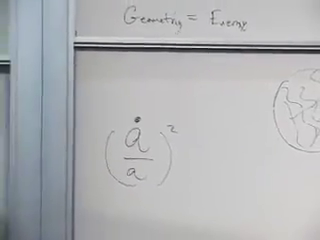
\includegraphics[width=0.68\textwidth]{lecture_06_figure_03.png}
\lectureframe{01:06:37.088}
\caption{Khẩu hiệu định hướng \emph{hình học bằng năng lượng}, với hạng giãn nở \(H^2=(\dot a/a)^2\) được viết bên dưới.}
\end{figure}

Đối với một vũ trụ đồng nhất và đẳng hướng, phương trình Friedmann thứ nhất là
\begin{equation}
H^2+\frac{k}{a^2}
=\frac{8\pi G}{3}\rho,
\end{equation}
trong đơn vị \(c=1\), trong đó \(k=+1,0,-1\) biểu thị hình học không gian đóng, phẳng hoặc mở và
\begin{equation}
\rho
=\rho_{\mathrm{ordinary}}
+\rho_{\mathrm{dark}}
+\rho_{\mathrm{radiation}}
+\rho_{\mathrm{vacuum}}.
\end{equation}
Dấu xuất hiện cạnh \(1/a^2\) phụ thuộc vào việc hạng độ cong được giữ ở vế trái hay chuyển sang vế phải, cũng như vào giá trị của \(k\).

\begin{figure}[H]
\centering
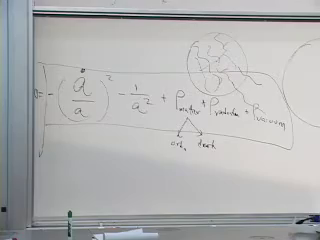
\includegraphics[width=0.96\textwidth]{lecture_06_figure_04.png}
\lectureframe{01:08:46.794}
\caption{Sự cân bằng đầy đủ trên bảng: giãn nở và độ cong không gian ở phía hình học, còn vật chất, bức xạ và năng lượng chân không ở phía nguồn. Vật chất còn được tách thêm thành các thành phần thường và tối.}
\end{figure}

\subsection{Ràng buộc Hamiltonian vũ trụ học}

\begin{classroomqa}
\audiencequestion{Nếu năng lượng chân không trong một vùng đồng chuyển động tăng lên khi vũ trụ giãn nở, thì có một mật độ năng lượng ròng không đổi hay một tổng năng lượng được bảo toàn không? \lecturetimestamp{01:01:51}}
\lecturerresponse{Thuyết tương đối rộng không cung cấp một năng lượng toàn cục phổ quát cho một không-thời gian giãn nở tùy ý. Tuy nhiên, trong phép rút gọn vũ trụ học đồng nhất, phương trình Einstein thành phần thời-thời là một ràng buộc Hamiltonian. Khi hình học và vật chất được đưa về cùng một vế, Hamiltonian chịu ràng buộc ấy bằng không. Các hạng vật chất đang biến đổi được cân bằng bởi các bậc tự do hấp dẫn, chứ không phải bởi một năng lượng cố định thông thường trong một cái hộp.}
\end{classroomqa}

Dưới dạng sơ đồ, phát biểu chính tắc là
\begin{equation}
\mathcal H_{\mathrm{gravity}}
+\mathcal H_{\mathrm{matter}}
=0.
\end{equation}
Đây là ý nghĩa chính xác của câu nói rằng tổng năng lượng bằng không. Đó là một phương trình chuyển động được áp đặt bởi tính bất biến đối với tái tham số hóa thời gian, chứ không phải là khẳng định rằng mọi mật độ năng lượng cục bộ đều triệt tiêu. Trong một thể tích đồng chuyển động, năng lượng của vật chất thông thường xấp xỉ cố định, năng lượng bức xạ giảm xuống, còn năng lượng chân không tăng lên; đồng thời, phần đóng góp hấp dẫn và tốc độ giãn nở tự điều chỉnh để ràng buộc của Einstein vẫn được thỏa mãn.

Bảo toàn cục bộ vẫn chính xác:
\begin{equation}
\nabla_\mu T^{\mu\nu}=0.
\end{equation}
Đối với chất lưu đồng nhất, đây chính là phương trình liên tục
\(\dot\rho+3H(\rho+p)=0\). Điều nói chung không còn đúng là trực giác từ không-thời gian phẳng cho rằng cũng phải tồn tại một tổng toàn cục của năng lượng vật chất, độc lập tọa độ, được bảo toàn trong một vũ trụ giãn nở.\editorialnote{Phân biệt này làm cho phát biểu trên lớp rằng năng lượng luôn bằng không trở nên chính xác: bảo toàn hiệp biến cục bộ và ràng buộc Hamiltonian vũ trụ học là chính xác, còn một năng lượng toàn cục duy nhất của vật chất cộng hấp dẫn thì nói chung không được định nghĩa.}

\begin{classroomqa}
\audiencequestion{Ràng buộc bằng không có phải là điều kiện quyết định vũ trụ là mở, đóng hay phẳng không? \lecturetimestamp{01:04:42}}
\lecturerresponse{Không. Ràng buộc Hamiltonian áp dụng trong mọi trường hợp. Các vũ trụ mở, phẳng và đóng khác nhau qua nhãn độ cong \(k\) và vì vậy qua hạng \(k/a^2\). Độ cong làm thay đổi một đóng góp trong sự cân bằng; nó không làm cho ràng buộc ấy có hiệu lực hay mất hiệu lực.}
\end{classroomqa}

\section{Tọa độ Grassmann và siêu trường}

\begin{classroomqa}
\audiencequestion{Các số Grassmann có thật sự xuất hiện trong Lagrangian của lý thuyết không? \lecturetimestamp{01:09:37}}
\lecturerresponse{Trước hết chúng xuất hiện vì các trường fermion là lẻ Grassmann. Chúng xuất hiện lần thứ hai như các tọa độ của siêu không gian. Các siêu trường phụ thuộc vào các tọa độ lẻ đó, và các tác dụng siêu đối xứng được xây dựng bằng cách lấy đạo hàm và tích phân theo chúng.}
\end{classroomqa}

Một trường thông thường là một hàm của không-thời gian,
\begin{equation}
\phi=\phi(x^\mu).
\end{equation}
Siêu đối xứng tối thiểu trong bốn chiều mở rộng \(x^\mu\) bằng một spinor lẻ hai thành phần \(\theta^\alpha\) và liên hợp của nó \(\bar\theta^{\dot\alpha}\):
\begin{equation}
z^M=(x^\mu,\theta^\alpha,\bar\theta^{\dot\alpha}).
\end{equation}
Có hai thành phần lẻ phức, hay bốn hướng lẻ thực. Một siêu trường là một hàm trên siêu không gian này:
\begin{equation}
\Phi=\Phi(x,\theta,\bar\theta).
\end{equation}

Đây không phải là những chiều không gian cực nhỏ theo nghĩa metric. Một tọa độ Grassmann không có độ lớn số học dương. Việc gọi nó là nhỏ chỉ là một cách gợi nhớ đến tính lũy linh:
\begin{equation}
(\theta^\alpha)^2=0,
\qquad
\theta^\alpha\theta^\beta=-\theta^\beta\theta^\alpha.
\end{equation}
\editorialnote{Chính tính lũy linh, chứ không phải sự nhỏ theo trị số, là lý do mọi khai triển theo một số hữu hạn tọa độ Grassmann đều kết thúc.}

Với bốn tọa độ lẻ độc lập, một siêu trường hoàn toàn tổng quát có nhiều nhất \(2^4=16\) đơn thức Grassmann. Dưới dạng sơ đồ,
\begin{equation}
\begin{aligned}
\Phi(x,\Theta)={}&\phi(x)+\Theta_A\psi_A(x)\\
&+\frac{1}{2}\Theta_A\Theta_B Z_{AB}(x)+\cdots\\
&+\Theta_1\Theta_2\Theta_3\Theta_4D(x),
\end{aligned}
\end{equation}
trong đó \(\Theta_A\) ký hiệu gộp cho bốn tọa độ lẻ thực. Vì toàn bộ siêu trường có thể được chọn là chẵn, nên các hệ số của những hạng bậc chẵn là bosonic còn các hệ số của những hạng bậc lẻ là fermionic. Vì thế, một siêu trường gói gọn một đa bội hữu hạn các trường thành phần thông thường.

Cách gói gọn này không chỉ là ký hiệu. Siêu đối xứng tác động về mặt hình học như một phép tịnh tiến theo các hướng lẻ đan xen với phép tịnh tiến trong không-thời gian. Một Lagrangian được xây dựng từ các siêu trường theo các quy tắc của siêu không gian sẽ thừa hưởng đối xứng đó theo cùng cách mà một Lagrangian vô hướng được xây dựng từ các tensor thừa hưởng tính bất biến quay hay Lorentz.

Tác dụng bây giờ bao gồm các độ đo Grassmann. Một hạng điển hình trên toàn siêu không gian có dạng
\begin{equation}
S_D=\int d^4x\,d^2\theta\,d^2\bar\theta\,
\mathcal K(\Phi,\Phi^\dagger).
\end{equation}
Còn các hạng chiral thì dùng
\begin{equation}
S_F=\int d^4x\,d^2\theta\,W(\Phi)+\mathrm{h.c.}
\end{equation}
\editorialnote{Sự phân biệt giữa độ đo trên toàn siêu không gian và độ đo chiral là sự tinh chỉnh tiêu chuẩn của tác dụng sơ đồ \(d^4x\,d^4\theta\). Các ví dụ cụ thể sẽ quyết định độ đo nào là thích hợp.}

Vì thế, ta đã đi tới một câu hỏi mà phép tính thông thường không trả lời được: tích phân trên một tọa độ phản giao hoán có nghĩa là gì?

\section{Tích phân Berezin}

\subsection{Mô hình thông thường: một đạo hàm toàn phần}

Hãy bắt đầu với một hàm thông thường \(F(x)\) triệt tiêu khi \(x\) dương rất lớn và âm rất lớn. Định lý cơ bản của giải tích cho
\begin{equation}
\int_{-\infty}^{\infty}dx\,\frac{dF}{dx}
=F(\infty)-F(-\infty)
=0.
\end{equation}

\begin{figure}[H]
\centering
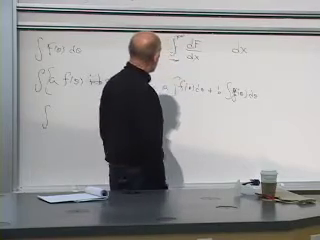
\includegraphics[width=0.88\textwidth]{lecture_06_figure_05.png}
\lectureframe{01:26:31.594}
\caption{Mẫu hình thông thường cho tích phân Berezin: tích phân của một đạo hàm toàn phần rút về các giá trị ở đầu mút và bằng không khi hàm tắt dần. Dòng phía dưới trên bảng bị che khuất một phần, nên phương trình rõ ràng được cung cấp trong phần văn bản.}
\end{figure}

Ta muốn tích phân Grassmann là tuyến tính và có chung tính chất hữu ích là tích phân của một đạo hàm toàn phần bằng không. Với một tọa độ lẻ, hãy yêu cầu
\begin{align}
\int d\theta\,[af(\theta)+bg(\theta)]
&=
a\int d\theta\,f(\theta)
+b\int d\theta\,g(\theta),\\
\int d\theta\,\partial_\theta f(\theta)&=0.
\end{align}
Điều kiện thứ hai là phép tương tự đại số của tính bất biến tịnh tiến của độ đo. Không có các đầu mút của một trục số lẻ, cũng không có tổng trên những khoảng cực nhỏ.

\begin{classroomqa}
\audiencequestion{Nếu không có tích phân Grassmann bất định, có phải ta đang từ bỏ ý tưởng rằng tích phân là phép nghịch đảo của đạo hàm không? \lecturetimestamp{01:21:19}}
\lecturerresponse{Vâng. Tích phân Berezin là một phiếm hàm tuyến tính xác định, không phải một phép lấy nguyên hàm. Với một biến Grassmann, trên thực tế nó được biểu diễn bởi cùng một phép toán đại số như phép đạo hàm.}
\end{classroomqa}

\begin{classroomqa}
\audiencequestion{Phép tích phân \(d^4x\) trên toàn bộ không-thời gian cũng là một tích phân xác định phải không? \lecturetimestamp{01:21:34}}
\lecturerresponse{Có. Khi người ta tích phân tác dụng trên không-thời gian, các điều kiện biên được hiểu ngầm. Khác biệt là tích phân thông thường trên không-thời gian có thể được hiểu qua giới hạn của các tổng, còn tích phân Grassmann được định nghĩa đại số bằng tác dụng của nó lên cơ sở hữu hạn \(1,\theta\).}
\end{classroomqa}

\subsection{Một biến}

Mọi hàm của một biến lẻ đều có thể được viết với hệ số ở bên phải theo thứ tự cố định
\begin{equation}
f(\theta)=a+\theta b.
\end{equation}
Vì \(\partial_\theta\theta=1\), quy tắc đạo hàm toàn phần suy ra
\begin{equation}
\int d\theta\,1=0.
\end{equation}
Chuẩn hóa còn lại được chọn là
\begin{equation}
\int d\theta\,\theta=1.
\end{equation}
Do đó,
\begin{equation}
\int d\theta\,f(\theta)=b.
\end{equation}
Tích phân chọn ra hệ số của lũy thừa cao nhất có thể có. Với quy ước đạo hàm trái dùng ở đây,
\begin{equation}
\partial_\theta f=b
=\int d\theta\,f.
\end{equation}

\begin{classroomqa}
\audiencequestion{Có tồn tại một hàm \(F(\theta)\) thỏa mãn \(\partial_\theta F=\theta\) không? \lecturetimestamp{01:30:05}}
\lecturerresponse{Không. Một hàm như vậy sẽ cần một hạng tỉ lệ với \(\theta^2\), nhưng \(\theta^2=0\). Đây là một cách khác để thấy vì sao không có tương tự Grassmann của một nguyên hàm bất định.}
\end{classroomqa}

\subsection{Hai biến và thứ tự của độ đo}

Đối với một cặp phức \(\theta,\bar\theta\), hãy viết một hàm chẵn tổng quát dưới dạng có thứ tự
\begin{equation}
f(\theta,\bar\theta)
=a+\bar\theta\psi+\bar\psi\theta+b\,\bar\theta\theta.
\end{equation}
Không có hạng bậc cao hơn nào vì
\begin{equation}
\theta^2=\bar\theta^2=0,
\qquad
\bar\theta\theta=-\theta\bar\theta.
\end{equation}

Bây giờ ta cố định quy ước
\begin{equation}
\int d\theta\,d\bar\theta\,
\bar\theta\theta=1.
\end{equation}
Với các tích phân lặp, phép toán \(d\bar\theta\) liền kề tác dụng trước. Khi đó bảng là
\begin{align}
\int d\theta\,d\bar\theta\,1&=0,\\
\int d\theta\,d\bar\theta\,\theta&=0,\\
\int d\theta\,d\bar\theta\,\bar\theta&=0,\\
\int d\theta\,d\bar\theta\,\bar\theta\theta&=1.
\end{align}
Do đó
\begin{equation}
\int d\theta\,d\bar\theta\,
f(\theta,\bar\theta)=b.
\end{equation}

\begin{classroomqa}
\audiencequestion{Đối với một hạng tuyến tính theo \(\theta\), có thật chính phép tích phân theo \(\theta\) làm cho tích phân kép triệt tiêu không? \lecturetimestamp{01:34:59}}
\lecturerresponse{Không; lời giải thích trực tiếp trên lớp đã đảo ngược vai trò của chúng. Tích phân \(\theta\) theo \(\theta\) cho ra 1. Khi đó kết quả không còn chứa \(\bar\theta\), và tích phân \(\bar\theta\) còn lại của 1 thì bằng không. Dù theo cách nào đi nữa, một tích phân kép chỉ còn lại khi cả hai biến đều hiện diện.}
\end{classroomqa}

\begin{classroomqa}
\audiencequestion{Nếu hoán đổi \(\theta\) và \(\bar\theta\), tích phân có đổi dấu không? \lecturetimestamp{01:36:33}}
\lecturerresponse{Có. Các biến lẻ và các độ đo lẻ phản giao hoán. Với quy ước ở trên,
\[
\int d\bar\theta\,d\theta\,\bar\theta\theta=-1.
\]
Vì thế, ta phải chọn một thứ tự và giữ nó nhất quán. Vật lý không phụ thuộc quy ước, nhưng các dấu trung gian thì có.}
\end{classroomqa}

Đối với \(n\) biến Grassmann độc lập, khuôn mẫu là hiển nhiên:
\begin{equation}
\int d\theta_n\cdots d\theta_1\,
f(\theta_1,\ldots,\theta_n)
\end{equation}
trích ra hệ số của đơn thức bậc cao nhất có thứ tự \(\theta_1\cdots\theta_n\), tới dấu được cố định bởi thứ tự đã chọn của các biến và các độ đo. Quy tắc trích xuất thành phần đơn giản này là động cơ đứng sau các tác dụng trên siêu không gian. Một biến thiên siêu đối xứng trở thành một đạo hàm toàn phần lẻ, và tích phân trên siêu không gian loại bỏ nó, cũng như một tác dụng thông thường loại bỏ một đạo hàm toàn phần theo không-thời gian dưới các điều kiện biên thích hợp.

\section{Vì sao một phép tính nhỏ như vậy lại có sức mạnh lớn đến thế}

Các quy tắc trông gần như tầm thường:
\begin{equation}
\int d\theta\,1=0,
\qquad
\int d\theta\,\theta=1.
\end{equation}
Thế nhưng chúng cho phép ta xây dựng các lý thuyết trường tương tác trong đó các quan hệ giữa các khối lượng bosonic và fermionic, cũng như giữa các hằng số ghép bosonic và fermionic, được duy trì tự động. Mục đích của phép tính trên siêu không gian cũng giống như mục đích của phép tính tensor trong thuyết tương đối: sắp xếp ký hiệu sao cho đối xứng mong muốn được duy trì qua mọi thao tác được phép.

Cái giá phải trả là việc theo dõi dấu. Mỗi lần hoán đổi hai đối tượng lẻ đều đóng góp một dấu trừ, và một phép tính có thể đúng về mặt ý niệm mà vẫn sai chỉ vì một lựa chọn thứ tự. Khó khăn đó không phải là thứ trang trí; nó là cái bóng đại số của thống kê fermion.

\begin{classroomqa}
\audiencequestion{Các số Grassmann được phát minh cùng với siêu đối xứng, hay chúng đã tồn tại từ trước? \lecturetimestamp{01:41:19}}
\lecturerresponse{Chúng lâu đời hơn rất nhiều. Hermann Grassmann đã phát triển đại số ngoại nền tảng ấy vào thế kỷ XIX. Các dạng vi phân vốn đã dùng các phần tử cơ sở phản giao hoán; lý thuyết trường lượng tử thế kỷ XX và siêu đối xứng đã tìm thấy một vai trò vật lý mới cho chính toán học đó.}
\end{classroomqa}

Giờ đây ta đã sẵn sàng cho những xây dựng cụ thể. Các siêu trường gom các đa bội boson-fermion đầy đủ, các đạo hàm trên siêu không gian bảo toàn đại số, và tích phân Berezin trích ra tác dụng thành phần. Nhiệm vụ tiếp theo là dùng bộ công cụ này trong mô hình một chiều đơn giản nhất rồi đưa nó vào lý thuyết trường.
